
%----------------------------------------------------------------------------------------
%  Multithreaded file tokenizer
%----------------------------------------------------------------------------------------

\section{Multi-threaded file tokenizer}

\subsection{Run with 2 threads and the input file provided. Does the code run exhibiting the desired
behaviour?}

The code does not exhibit the correct behaviour because the threads are not tokenizing the lines in a
round-robin fashion. This cause unbalanced loading of work for each threads and means that some thread may
be idle waiting for work. This is exactly the case as seen in \cref{fig:lab2part3}, only a single line
is allocated to thread1, and the rest of the lines in the file is allocated to thread0 to tokenize.

\begin{figure}[ht]
    \centering
    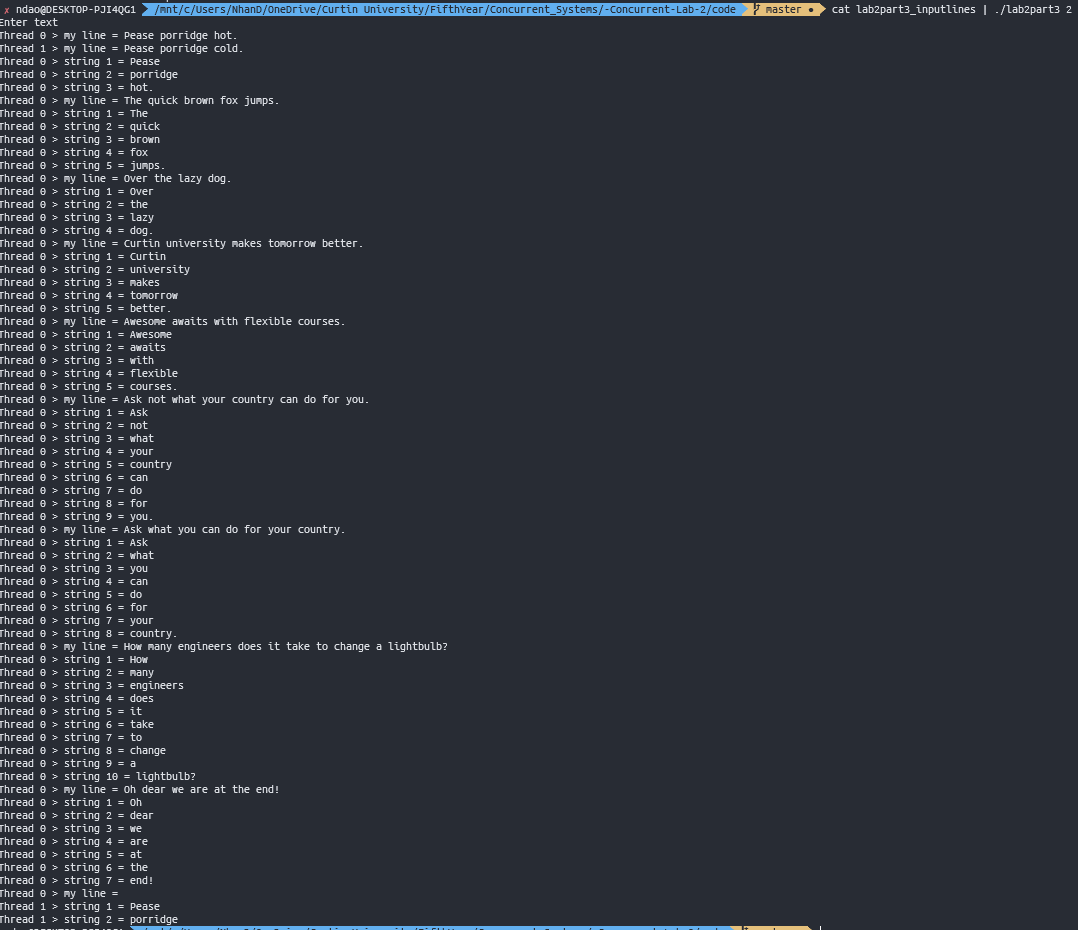
\includegraphics[width=\textwidth]{Figures/part3_2.PNG}
    \caption{Terminal output of lab2part3.c program using 3 threads and lab2part3\_inputlines as input}
    \label{fig:lab2part3}
\end{figure}

\subsection{Inital value of samaphores for each thread}

The number of semaphores are the same as the number of threads created using an $n$ array (sem\_t) array
where $n$ is the number of threads. The first semaphore in position $0$ is initialized to 1 and the rest
are intialized to 0, see \cref{lst:lab2part3a}.

\pagebreak
\vspace{0.5cm}
\lstinputlisting[
	style=CStyle,
	firstline=37, % First line of code
	lastline=40, % Lastl ine of code
	caption=Initial values for each semaphores for each thread (line 37-40 in lab2part3.c), % Caption above the listing
	label=lst:lab2part3a, % Label for referencing this listing
	frame=single, % Frame around the code listing
	showstringspaces=false, % Don't put marks in string spaces
	numbers=left, % Line numbers on left
	numberstyle=\normalsize % Line numbers styling
    ]{../code/lab2part3.c}

%----------------------------------------------------------------------------------------

\subsection{Modifying \emph{Tokenize} function to achieve the desired behaviour}

To allow for the threads to read each line of the file in a round-robin fashion, semaphores can be used
to synchronise the thread. Essentially, a thread with rank $i$ call \emph{sem\_wait} on semaphore $i$ before
entering the critical section, which is reading the new line from the file pointer and executing the 
tokenizer. Then it calls \emph{sem\_post} on sem $i+1$, which means that the thread with rank $i+1$ can 
grab the nextline, (modulo the result by the total thread count to wrap the largest rank thread
back to the thread with rank 0). \Cref{lst:lab2part3b}, shows the section of code in \emph{Tokenize} that
performs the load balancing.

\pagebreak
\vspace{0.5cm}
\lstinputlisting[
	style=CStyle,
	firstline=131, % First line of code
	lastline=151, % Lastl ine of code
	caption= Thread syncrhonsation using semaphores for load balancing (line 131-151 in lab2part3.c), % Caption above the listing
	label=lst:lab2part3b, % Label for referencing this listing
	frame=single, % Frame around the code listing
	showstringspaces=false, % Don't put marks in string spaces
	numbers=left, % Line numbers on left
	numberstyle=\normalsize % Line numbers styling
    ]{../code/lab2part3.c}

